\documentclass[12pt,twoside]{article}
\usepackage{amsmath}

\usepackage{times}
\usepackage{helvet}

%\usepackage{fontspec}
%\setmainfont{Liberation Serif}
%\setsansfont{Liberation Sans}

\usepackage{geometry}
\geometry{               
	letterpaper,
	bottom=0.5in,
	top=0.5in,
	inner=1in,
	outer=0.5in,
        footskip=4ex
}

\usepackage{graphicx}

\usepackage{titling}
\pretitle{\begin{center}\LARGE\sffamily}
\posttitle{\par\end{center}\vspace{-4ex}}
\preauthor{\begin{center}\large\sffamily}
\postauthor{\par\end{center}\vspace{-12ex}}
\setlength{\droptitle}{-60pt}



\usepackage{multienum}

\usepackage{titlesec}
\titleformat*{\section}{\Large\sffamily}
\titleformat*{\subsection}{\sffamily}

\titlespacing\section{2em}{0.5ex plus 0.2ex minus 0.1ex}{0pt}
\titlespacing\subsection{1em}{0.5ex plus 0.2ex minus 0.1ex}{0pt}

\usepackage{fancyhdr}
\pagestyle{fancy}

\fancyhf{}
\renewcommand{\headrule}{}
\fancyfoot[LE]{\thepage}
\fancyfoot[RO]{\thepage}

\usepackage{multicol}

\setlength{\parindent}{0pt}

\fancyfoot[C]{\tiny \begin{tabular}[b]{c}
    Remixed from \textit{Prealgebra 2e} by Lynn Marecek, MaryAnne Anthony-Smith, Andrea Honeycutt Mathis \\
    Access for free at https://openstax.org/books/prealgebra-2e/pages/1-introduction
\end{tabular}}


\title{Lesson 1}
\author{Foundations of College Algebra}
\date{}

\begin{document}

\maketitle

\thispagestyle{fancy}

\section*{Exponential Notation}

\subsection*{Definitions}
For any expression $a^n$, $a$ is a factor multiplied by itself $n$ times if $n$ is a positive integer. That is
$$a ^n = \underbrace{a \cdot a \cdot \dots \cdot a}_{n \text{ times}}.$$
The number $a$ is the \textbf{base} and the number $n$ is the \textbf{exponent}.

\subsection*{Examples}

Write each expression in exponential form.
\begin{multienumerate}
  \mitemxxx{$9\cdot 9 \cdot 9 \cdot 9 \cdot 9$}
           {$16 \cdot 16 \cdot 16 \cdot 16 \cdot 16 \cdot 16 \cdot 16$}
           {$4 \cdot 4 \cdot 4 \cdot 5 \cdot 5 \cdot 7 \cdot 7 \cdot 7 \cdot 7$}
\end{multienumerate}

Write each exponential expression in standard form.
\begin{enumerate}
  \item $8^6$
\end{enumerate}

Simplify the following.
\begin{multienumerate}
  \mitemxxx{$3 ^ 4$}{$4 ^ 3$}{$2^3 \cdot 3 ^ 2$}
\end{multienumerate}

\subsection*{You Try}

Write each expression in exponential form.
\begin{multienumerate}
  \mitemxxx{$7 \cdot 7 \cdot 7 \cdot 7 \cdot 7 \cdot 7 \cdot 7 \cdot 7 \cdot 7$}
           {$41 \cdot 41 \cdot 41 \cdot 41 \cdot 41$}
           {$3 \cdot 3 \cdot 4 \cdot 4 \cdot 12 \cdot 12 \cdot 12 \cdot 12$}
\end{multienumerate} \vspace\fill

Write each exponential expression in standard form.
\begin{enumerate}
  \item $4^8$
\end{enumerate} \vspace\fill

Simplify the following.
\begin{multienumerate}
  \mitemxx{$7^2$}{$5^3$} \vspace\fill
  \mitemxx{$1^9$}{$4^2\cdot3^2$} \vspace\fill
\end{multienumerate}

\pagebreak

\section*{Square Roots}

\subsection*{Definition}

\begin{itemize}\itemsep=-\parsep
\item A number whose square is $m$ is called a \textbf{square root} of $m$. That is, if $n^2 = m$, then $n$ is a square root of $m$.
\item Every positive number has two square roots: one positive and one negative.
\item The positive square root is called the \textbf{principle square root} is denoted with a \textbf{radical sign}: $\sqrt{m}$.
\end{itemize}

\subsection*{Examples}
Simplify the following.
\begin{multienumerate}
  \mitemxx{$\sqrt{25}$}{$\sqrt{121}$}
\end{multienumerate}

\subsection*{You Try}
Simplify the following.
\begin{multienumerate}
  \mitemxx{$\sqrt{16}$}{$\sqrt{169}$}
\end{multienumerate} \vspace\fill

\section*{Order of Operations}

\subsection*{How To - Using the Order of Operations}
When simplifying mathematical expressions, perform the operations in the following order:
\begin{multicols}{2}
  \begin{enumerate}\itemsep=-\parsep
  \item \textbf{P}arentheses and grouping symbols, working on the innermost parentheses first.
  \item \textbf{E}xponents
    \columnbreak
  \item \textbf{M}ultiplication and \textbf{D}ivision left to right.
  \item \textbf{A}ddition and \textbf{S}ubtraction left to right.
    \end{enumerate}
\end{multicols}

\subsection*{Examples}
Simplify.
\begin{multienumerate}
  \mitemxx{$3 \cdot 8 - 5 \cdot 2$}{$20 \div 4 + 6 \cdot 5$}
  \mitemxx{$20 \div (4 + 6)\cdot5$}{$3(1 + 9 \cdot 6) - 4$}
\end{multienumerate}

\subsection*{You Try}
Simplify.
\begin{multienumerate}
  \mitemxx{$4 + 6 (3 + 6)$}{$6 + 10 \div 2 + 2$} \vspace\fill
  \mitemxx{$33 \div (3 + 8) \cdot 2$}{$5 \left[2 + 4 (3 - 2) \right]$} \vspace\fill
\end{multienumerate}

\pagebreak

\section*{Review of Fractions}

\subsection*{Definition}
\begin{itemize}\itemsep=-\parsep
\item A \textbf{fraction} is written $\frac{a}{b}$, where $a$ and $b$ are whole numbers and $b \neq 0$.
\item The \textbf{denominator} is the bottom number and tells how many parts make a whole.
\item The \textbf{numerator} is the top number and tells how many parts are in the measurement.
\end{itemize}

\subsection*{Division Properties}
\begin{multicols}{2}
  \begin{itemize}\itemsep=-\parsep
  \item Any number (except 0) divided by itself is 1.
  \item Any number divided by 1 is the same number.
  \item Zero divided by any number (except 0) is 0.
    \columnbreak
  \item Dividing a number (except 0) by 0 is undefined.
  \item Zero divided by zero is indeterminate.
  \end{itemize}
\end{multicols}

\section*{Mixed Numbers and Improper Fractions}

\subsection*{Definitions}

\begin{itemize}\itemsep=-\parsep
\item A fraction is a \textbf{proper fraction} if the numerator is less than the denominator.
\item A fraction is an \textbf{improper fraction} if the numerator is greater than or equal to the denominator.
\item A \textbf{mixed number} consists of a whole number and a proper fraction.
\end{itemize}

\subsection*{Examples}
Name the improper fraction. Write it as a mixed number.
\begin{multienumerate}
  \mitemxx{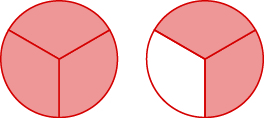
\includegraphics[width=0.33\textwidth]{Lesson_1_1.jpeg}}
  {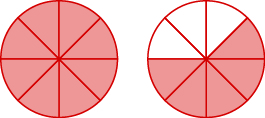
\includegraphics[width=0.33\textwidth]{Lesson_1_2.jpeg}}
\end{multienumerate}

\begin{multicols}{2}
  \subsection*{How To - Convert a Mixed Number to an Improper Fraction}
  \begin{enumerate}\itemsep=-\parsep
  \item Multiply the whole number by the denominator.
  \item Add the numerator to the product found in Step 1.
  \item Write the final sum over the original denominator.
  \end{enumerate}

  \subsection*{Examples}
  Convert the mixed numbers into improper fractions.
  \begin{multienumerate}
    \mitemxx{$ 10 \frac27$}{$ 4 \frac6{11}$}
  \end{multienumerate}

\subsection*{You Try}
  Convert the mixed numbers into improper fractions.
  \begin{multienumerate}
    \mitemxx{$ 1 \frac5{16}$}{$ 11 \frac13$}
  \end{multienumerate} \vspace\fill
  
  \columnbreak

  \subsection*{How To - Convert an Improper Fraction to a Mixed Number}
  \begin{enumerate}\itemsep=-\parsep
  \item Divide the denominator into the numerator.
  \item Identify the quotient, remainder, and divisor.
  \item Write the mixed number as
    $$ \text{quotient} \frac{\text{remainder}}{\text{divisor}}.$$
  \end{enumerate}

\subsection*{Examples}
  Convert the improper fractions into mixed numbers.
  \begin{multienumerate}
    \mitemxx{$\frac{33}8$}{$\frac{183}5$}
  \end{multienumerate}

\subsection*{You Try}
  Convert the improper fractions into mixed numbers.
  \begin{multienumerate}
    \mitemxx{$\frac{23}7$}{$\frac{48}{11}$}
  \end{multienumerate}
\end{multicols} \vspace\fill

\pagebreak

\section*{Prime Factorization}

\subsection*{Definitions}
\begin{itemize}\itemsep=-\parsep
\item When two numbers are multiplied together, each number is called a \textbf{factor}. The answer to the multiplication is called
  the \textbf{product}.
\item A \textbf{prime} number is a whole number greater than 1 whose only factors are 1 and itself.
\item A \textbf{composite} number is a whole number that is not prime.
\item The \textbf{prime factorization} of a number is the product of prime numbers that equals the number.
\end{itemize}

\subsection*{Examples}
Find all factors of the following numbers.
\begin{multienumerate}
\mitemxx{$22$}{$72$}
\end{multienumerate}

Identify the following numbers as either prime or composite.
\begin{multienumerate}
  \mitemxx{$83$}{$77$}
\end{multienumerate}

Find the prime factorization of the following numbers.
\begin{multienumerate}
  \mitemxxx{$36$}{$80$}{$588$}
\end{multienumerate}

\subsection*{You Try}
Find all factors of the following numbers.
\begin{multienumerate}
\mitemxx{$18$}{$96$} \vspace{0.75in}
\end{multienumerate}

Identify the following numbers as either prime or composite.
\begin{multienumerate}
  \mitemxx{$57$}{$91$} \vspace\fill
\end{multienumerate}

Find the prime factorization of the following numbers.
\begin{multienumerate}
  \mitemxxx{$48$}{$60$}{$126$} \vspace\fill
\end{multienumerate}

\end{document}
